\newpage
\section{Flabby Flame - Corona SDK\\ {\small \emph{Eduard Bicego}}}
\label{sec:corona}

	Ho strutturato questa sezione presentando inizialmente le mie impressioni sull'utilizzo delle librerie offerte da Corona SDK. In seguito ho descritto le impressioni dell'ambiente attorno allo sviluppo con Corona SDK. Infine le regole di usabilità rispettate nell'applicazione finale.
	Per quanto riguarda i test su dispositivo fisico sono stati fatti su un ASUS zenPhone Go con sistema operativo Android OS, pertanto non ho potuto avere un riscontro sulle funzionalità dell'applicazione anche su iOS.
	
	\subsection{Corona API}

	\subsubsection{Audio}
		Per quanto riguarda l'audio Corona offre una libreria intuitiva e facile. Attraverso le chiamate \verb|audio.loadStream()| e \verb|audio.loadSound()| è possibile caricare i file audio in memoria e riprodurli attraverso i semplici metodi \verb|play()|, \verb|pause()| e \verb|stop()|. Riguardo al metodo \verb|play()| è necessario dichiarare il canale nel quale l'audio sarà riprodotto, questa gestione è lasciata allo sviluppatore in questo modo si ha il totale controllo sull'interazione delle diverse tracce audio.
		
		Personalmente ho trovato facile usare la libreria e in pochi passi sono riuscito ad aggiungere le musiche al gioco. La difficoltà maggiore per giochi più avanzati potrebbe essere quella di gestire il corretto flusso delle musiche seguendo gli eventi.
		
		
		\paragraph{Problematiche}
			Non ho riscontrato nessuna problematica particolare. Ho preferito lavorare con il sonoro disattivato o a basso volume, questo per il fastidio del continuo riavvio e non per problematiche riguardanti Corona.
	
	\subsection{Composer}
		Il \verb|composer| è un'API che permette di gestire le scene del gioco, ossia le schermate, in modo modulare. Ogni scena si occupa di gestire 6 importanti eventi (fasi):
		\begin{enumerate}
			\item La \textbf{creazione} (\verb|create|);
			\item La \textbf{visualizzazione prossima} su schermo (\verb|show will|);
			\item La \textbf{visualizzazione} su schermo (\verb|show did|);
			\item La \textbf{sparizione prossima} dallo schermo (\verb|hide will|);
			\item La \textbf{sparizione} dallo schermo (\verb|hide did|);
			\item La \textbf{distruzione} (\verb|destroy|);
		\end{enumerate}
		La potenzialità di questa libreria è il fatto di incapsulare parti del gioco riutilizzabili in diversi momenti e con altre scene. Infatti ho potuto riutilizzare lo stesso menu della schermata iniziale per il menu di pausa. Interessante l'interazione con gli oggetti display e widget i quali sono automaticamente gestiti da essa nella rimozione dallo schermo se opportunamente inseriti nella scena.
		
		\paragraph{Problematiche}
		Avendo già un background nello sviluppo su Android con API native la libreria \verb|composer| è stata una piacevole sorpresa e ha velocizzato lo sviluppo. Infatti essa rimarca il concetto di \verb|Fragment| dell'Android SDK. Peccato che tali somiglianze le abbia scoperte solo grazie ai vari tentativi e fallimenti infatti molte cose non sono esplicitate nella documentazione. Ad esempio non è chiara la distinzione tra gli eventi \verb|will|/\verb|did| e nulla viene menzionato su quando sia corretto aggiungere/rimuovere i listener, quando aggiungere/rimuovere oggetti su schermo o musiche e altro.
		
		
	\subsection{Display}
		\verb|display| è sicuramente l'api più utilizzata ed infatti presenta numerosi metodi per ogni evenienza. Ogni oggetto su schermo viene creato da questi metodi: cerchi, rettangoli etc. Offre molte funzionalità per facilitare la componibilità di elementi grafici grazie a \verb|newGroup()| e \verb|newContainer()|. L'integrazione con la parte \verb|physics| è eccellente e verrà discussa in seguito. 
		
		\paragraph{Problematiche}
		Ho trovato molto difficile utilizzare i metodi con molti parametri, anche perché una volta scritto il metodo alla rilettura non ricordavo quale variabile corrispondesse con il parametro visto che spesso si usano direttamente numeri per indicare le coordinate di un elemento grafico. A peggiorare la situazione c'è un'incoerenza nei metodi. Infatti i parametri variano spesso di posizione: \verb|display.newImageRect(filename, width, height)| presenta una serie di parametri molto diversi da altri metodi.
		\begin{verbatim}
			local displayElem = display.newImageRect("img/img.png", 100, 100)
			displayElem.x = 10;
			displayElem.y = 10;
		\end{verbatim}
		
		Nel secondo invece per definire \verb|x| e \verb|y| basta la sola chiamata al metodo:
	
		\begin{verbatim}
			local displayElem = display.newRect(10, 10, 100, 100)
		\end{verbatim}
		
		Nel terzo invece bisogna elencare una tabella di opzioni:
		
		\begin{verbatim}
		local displayElem = display.newText(
		{
		text = "SCORE: " .. score,
		x = display.contentCenterX,
		y = bottomRightY - 15,
		font = native.systemFont,
		fontSize = 16,
		align = "center"
		})
		\end{verbatim}
		
		Come si vede lo sviluppatore deve ricordarsi ben 3 modi diversi per creare elementi sullo schermo. Personalmente dove possibile ho sempre preferito la terza scrittura la quale risulta estremamente più leggibile della seconda e della prima chiamata a metodo.
		Anche in questo caso la documentazione approfondita non esiste o è carente. Mi sono trovato molte volte a creare parti di codice solo per test di alcune funzionalità.
		
		
	\subsection{Json}
		Per il salvataggio di dati dell'utente è possibile utilizzare un file json e la libreria dedicata \verb|json|. Esiste la possibilità di creare un database SQLite ma per le ridotte esigenze del gioco ho preferito limitarmi ad usare un semplice file json.
		
		\paragraph{Problematiche}
			Non ho notato particolari criticità per questa parte. La lettura e scrittura è molto semplice ma molto meccanica e quindi a rischio di stupidi errori. Per evitare questo ho scritto un piccolo file \verb|JsonUtils| che racchiude le funzioni necessarie per recuperare i dati salvati.
		
	\subsection{Physics}
		\verb|physics| è una libreria che collega gli oggetti \verb|displayObject| al motore fisico 2Dbox. Ho utilizzato la fisica solo per la palla di fuoco mossa dal giocatore. Aggiungere la fisica ad un oggetto è semplice \verb|physics.addBody()| e lo stesso per rimuoverla asta \verb|physics.removeBody()|. La costruzione di corpi fisici diversi da cerchi e rettangolo risulta più ostica e per le stalattiti ho dovuto tentare più volte per capire se ero riuscito a creare un corpo triangolare. Fortunatamente esiste la funzione di debug \verb|physics.setDrawMode("hybrid")| che permette di visualizzare sia gli oggetti grafici sia i corpi fisici collegati ad esso.
		
		\paragraph{Problematiche}
		Purtroppo gli oggetti a cui è applicata la fisica non sono componibili e quindi non sono riuscito ad implementare la fiamma che dovrebbe comparire quando l'utente 
		tocca lo schermo per saltare.
		
	\subsection{Widget}
		Mi sono servito della libreria \verb|widget| nella costruzione dei pulsanti e slider dei menu e sottomenu. 
	
		\paragraph{Problematiche}
		La libreria widget risulta essere la parte più deludente vista di Corona SDK. Le opzioni sono minimali e tutto il lavoro di design e stile dei widget è lasciato al programmatore. Infatti negli esempi e tutorial che ho trovato si preferisce sempre creare tutto con software grafici e poi utilizzare \verb|display.newImageRect()| piuttosto di appoggiarsi a questa libreria. La mancanza di un oggetto \verb|Layout| e tutti i suoi derivati è la cosa più grave. Nel mio caso avendo per ogni pulsante del menu delle coordinate assolute rispetto allo schermo mi sono risultati ostici semplici aggiunte o rimozioni di pulsanti o ancora più semplicemente la semplice modifica di un pulsante. Tutto infatti andava riposizionato da capo. Ho dovuto creare da zero delle funzioni di calcolo per mantenere le proporzioni nel caso avessi cambiato anche solo la dimensione di un pulsante di 1px. 
		Per questa esperienza sconsiglio il framework Corona per applicazioni di tipo business.
	
	\subsection{Ambiente di sviluppo}
	
		\subsubsection{Lua}
			Nonostante il linguaggio sia promosso come un linguaggio facile ho trovato molte difficoltà iniziali soprattutto nello strutturare e organizzare il codice. Penso che questo derivi dal mio background in cui prevale la conoscenza della programmazione orientata a orientati ad oggetti e non prototype-based come Lua. Una volta superato questo gradino iniziale non ho avuto più ostacoli di questo genere.
		
		\subsubsection{Debug e Simulatore}
			Il simulatore è certamente lo strumento più potente fornito dal framework. Veloce e immediato, il riavvio del gioco dopo le modifiche ai file lua velocizzano ancor di più lo sviluppo. Personalmente mi sono trovato molto bene. Dall'altra parte la console seppur spartana nell'aspetto dà allo sviluppatore tutto il necessario. 
	
		\subsubsection{Editor Atom}
			Seguendo i consigli nel forum di Corona ho installato e utilizzato l'editor Atom esteso con il plugin per Corona SDK. Sull'editor ho poco da dire, simile alle controparti Visual Studio Code o Brackets etc. Fa il suo lavoro, ottima l'integrazione con git.
			
			Riguardo al plugin per corona invece sono rimasto molto deluso, l'unica funzionalità che dà è un menu a tendina per scegliere le funzioni dalle componenti della libreria prima presentate. Non c'è modo di vedere la documentazione direttamente nell'editor. Addirittura anche la scelta dei metodi dal menu a tendina costringe quasi sempre a dover aprire il browser e cercare la documentazione del relativo metodo. Nella figura\ref{fig:atomPlugin} si vede come il plugin non offra nessuna spiegazione per i parametri richiesti dal metodo \verb|composer.gotoScene()|.
			
			Trovo assolutamente necessario per il futuro di corona una più stretta collaborazione per incorporare il simulatore, la console e la fruizione della documentazione direttamente nell'editor Atom o qualsiasi altro editor valido.
			
			\begin{figure} [t]
				\centering
				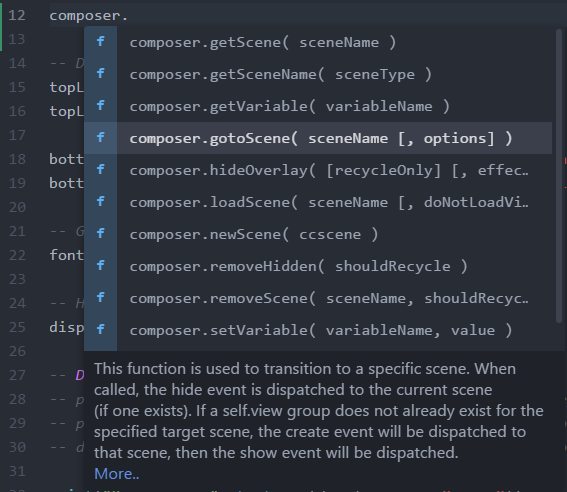
\includegraphics[width=0.8\textwidth]{img/atomPlugin}
				\caption{L'aiuto blando offerto dal plugin Corona per Atom}
				\label{fig:atomPlugin}
			\end{figure}
		
		\subsection{Build}
			Riguardo la compilazione dell'applicazione non ho avuto particolari problemi se non che è risultata dipendente dalla connessione a Internet e quindi il più delle volte lenta. 
	
	
	\subsection{Usabilità}
				
		\paragraph{Gioco}
			Nel gioco viene introdotto attraverso un piccolo tutorial introduttivo all'avvio del gioco. Il gioco infatti pretende che l'utente fin da subito prema sullo schermo per mantenere in volo la palla. Ho scelto di tenere il tutorial permanente finché l'utente non prenda un punto. In questo modo si ha la certezza che l'utente l'abbia letto almeno una volta e sappia come giocare. Facendo così evito il disorientamento e la frustrazione dell'utente ai primi game over.
			
			Il gioco funziona solo in posizione landscape left, in questo modo il pulsante di Pausa del gioco nella versione Android non si trova vicino ai pulsanti di sistema. Il gioco scorre da destra verso sinistra quindi l'utente sarà più propenso a giocare con la mano sinistra. Questo ragionamento ha fatto sì che il pulsante fosse posizionato a sinistra mentre è stata scelta la posizione in alto perché l'area è più facile da raggiungere e non risulta coperta rispetto agli angoli inferiori.
		
			Il secondo tutorial implementato spiega il modo alternativo per mettere in pausa, ossia scuotendo il device. Questo tutorial viene presentato solo quando l'utente preme per la prima volta il pulsante Pausa. Questa funzionalità sperimentale è stata implementata principalmente per scopo didattico per testare l'uso dei sensori con Corona. L'implementazione del listener all'accelerometro è stato immediato e intuitivo.
		
		
		
		Il pulsante di pausa in gioco è situato in alto a sinistra, una zona
	
		\paragraph{Menu} Per quanto riguarda il menu si è optata la scelta di avere pulsanti grandi per facilitare la corretta pressione a scapito di avere più sotto menu. Il menu è situato sulla parte centrale dello schermo ossia la zona più facilmente raggiungibile dai pollici dell'utente. Per ridurre lo spazio occupato nello schermo si è optato per l'utilizzo di icone universalmente riconosciute per i seguenti sotto menu:
		\begin{itemize}
			\item Best score;
			\item Info;
		\end{itemize}
		Inoltre ogni sotto menu presenta il pulsante BACK il quale si trova al centro dello schermo e consente all'utente una veloce navigazione e esplorazione dei vari sotto menu.
		
		Il pulsante Exit precedentemente implementato è stato rimosso perché ritenuto inutile in ambito mobile visto che solitamente l'utente esce dall'app tramite il tasto Home. Anche l'opzione del Volume potrebbe essere rimossa visto che, sempre in ambito mobile, l'utente infatti è abituato a gestire l'audio tramite widget offerti dal sistema operativo.
		
		A seguito di tutto quello già descritto della scarsa libreria \verb|widget|, ritengo un compito arduo gestire la User Experience con Corona SDK.
	
		
	\subsection{Valutazione finale}
		Vantaggi:
		\begin{itemize}
			\item Simulatore immediato, essenziale e veloce.
			\item Lua è ottimo per chi proviene dal mondo Javascript e Python o è nuovo al mondo della programmazione;
			\item Buona la documentazione per iniziare, anche per totali inesperti;
			\item Ottime librerie per la gestione dell'audio, degli oggetti visualizzabili e per gestire la fisica del gioco.
			\item Multipiattaforma;
			\item Ottimo per iniziare a programmare in modo veloce videogame 2D;
			\item Gratuito, le applicazioni prodotte sono commercializzabili e non richiedono acquisti di licenza. Ci sono abbonamenti ma solo per avere altri strumenti di sviluppo più avanzati.
		\end{itemize}
		Svantaggi:
		\begin{itemize}
			\item Lua: per i programmatori abituati ai linguaggi orientati agli oggetti diventa una difficoltà in più perché gli è richiesto un cambio di approccio nella programmazione. Inoltre Lua è un linguaggio poco spendibile in altri contesti se non nello sviluppo di giochi.
			\item Insufficiente la documentazione per approfondire le potenzialità offerte dal framework.
			\item Mancanza di librerie per la gestione tipica di menu, manca l'implementazione di concetti come il layout. Tutto è posizionato nello schermo in coordinate assolute, ciò fa sì che una modifica richieda di cambiare anche tutte le posizioni degli elementi su schermo. Risulta quindi ostico gestire al meglio l'usabilità.
			\item Il framework è cross-platform ma resta comunque un engine per soli giochi 2D, difficile da utilizzare per altri tipi di applicazioni (vedi precedente svantaggio)
			\item Il framework supporta solo la costruzione di ambienti 2D.
			\item Mancanza di un editor di sviluppo ideato per Corona, si pensi ad Android Studio per Android o a Visual Studio per Xamarin o Unity. Esistono alcuni plugin per famosi editor ma non velocizzano molto la fase di codifica.
			\item Compilare la propria applicazione richiede una connessione Internet. È un processo che a lungo andare fa perdere molto tempo soprattutto quando si vuole ripetutamente testare sui device fisici, la dimensione del codice sorgente è notevole (pensiamo alle immagini) e/o la propria connessione è lenta.
		\end{itemize}
		
		
		\subsection{Considerazioni finali}
			Le principali difficoltà riscontrate nello sviluppo di Flappy Flame non devono ricadere al 100\% su Corona, la mia scarsa competenza di uso di un linguaggio di scripting e di sviluppo di videogame ha rallentato molto inizialmente lo sviluppo. Infatti lo sviluppo di un videogame presenta una moltitudine di problemi legati fra loro e spesso molto più complessi di un’applicazione business: la gestione del Game Loop ne è un esempio.
			
			Ritengo Corona un framework perfetto per avvicinarsi alla programmazione di videogame soprattutto per chi ha già un Javascript in background. Dall'altra parte vedo ardua la creazione di giochi molto complessi con Corona SDK e in quel caso mi cercherei altri framework più avanzati e complessi. Ritengo la totale gratuità un vantaggio notevole, soprattutto per il mondo degli sviluppatori indipendenti. 
			
			Dal lato dell'usabilità Corona SDK sembra non averci minimamente pensato, basti pensare alla lacunosa libreria \verb|widget| e ritengo Corona SDK un framework inappropriato per applicazioni con contesti non ludici.
			
			Corona ha certamente delle grandi potenzialità ma quello che secondo me fa la differenza nella scelta delle tecnologie è l’ambiente di sviluppo. Ritengo che questo sia un punto fondamentale per l’affermazione di un framework. La totale assenza di un editor integrato con tutti gli altri strumenti: simulatore, console, documentazione inline etc. fa sì che lo sviluppo con Corona SDK sia una quasi costante fonte di frustrazione.
			
			\paragraph{} Quindi: Corona SDK sì o no? Sì, se si è alle prime armi e si voglia sperimentare lo sviluppo di un videogame con budget limitato, no altrimenti.
			
		

